\documentclass[11pt]{article}
\usepackage[margin=0.68in]{geometry}
\usepackage{booktabs,enumitem,fancyhdr,graphicx,overpic,tabularx,titlesec}
\usepackage[table]{xcolor}
\usepackage[hidelinks]{hyperref}
\graphicspath{{docs/lessons/assets/}{../assets/}}
\hypersetup{pdftitle={ADK Lesson 041: Presence and Passage},
 pdfauthor={Kevin Shanahan},
 pdfsubject={Copied PIR, optical, and timed range evidence},
 pdflang={en-US}}
\pagestyle{fancy}\fancyhf{}
\lhead{\textsc{ADK Lesson 041}}\rhead{Presence and Passage}
\cfoot{\thepage}\setlength{\headheight}{14pt}
\setlength{\parindent}{0pt}\setlength{\parskip}{5pt}
\setlist{nosep,leftmargin=1.45em}
\titleformat{\section}{\Large\bfseries}{\thesection}{0.5em}{}
\newcommand{\lessonbox}[1]{\begin{center}\fbox{\parbox{0.92\linewidth}{#1}}\end{center}}

\begin{document}
\begin{center}
 {\Huge\bfseries Presence and Passage}\\[4pt]
 {\Large Preserve source identity, age, and disagreement}\\[8pt]
 \textit{Host-verified E0 replay; powered composition and bench gates remain open}
\end{center}
\begin{tabularx}{\linewidth}{@{}>{\bfseries}l X >{\bfseries}l X@{}}
Lesson & 041 --- component & Time & 120--180 minutes\\
Prerequisites & Lessons 019 and 040 & Board & synthetic Mega replay only\\
Evidence & D30 acquisition LED and D31 TP-PRESENCE LED &
Status & host verified E0; powered composition and bench open\\
\end{tabularx}

\lessonbox{\textbf{Scope gate.} This lesson composes supplied observations.
It publishes no supported sensor circuit, wiring table, formal schematic, or
powered adapter. Family names authorize planning only. It makes no lux,
distance-accuracy, occupancy, security, navigation, collision-avoidance,
traffic-enforcement, identity, or life-safety claim.}

\section{Keep four evidence lanes separate}
\begin{center}
% ADK visual: pencil
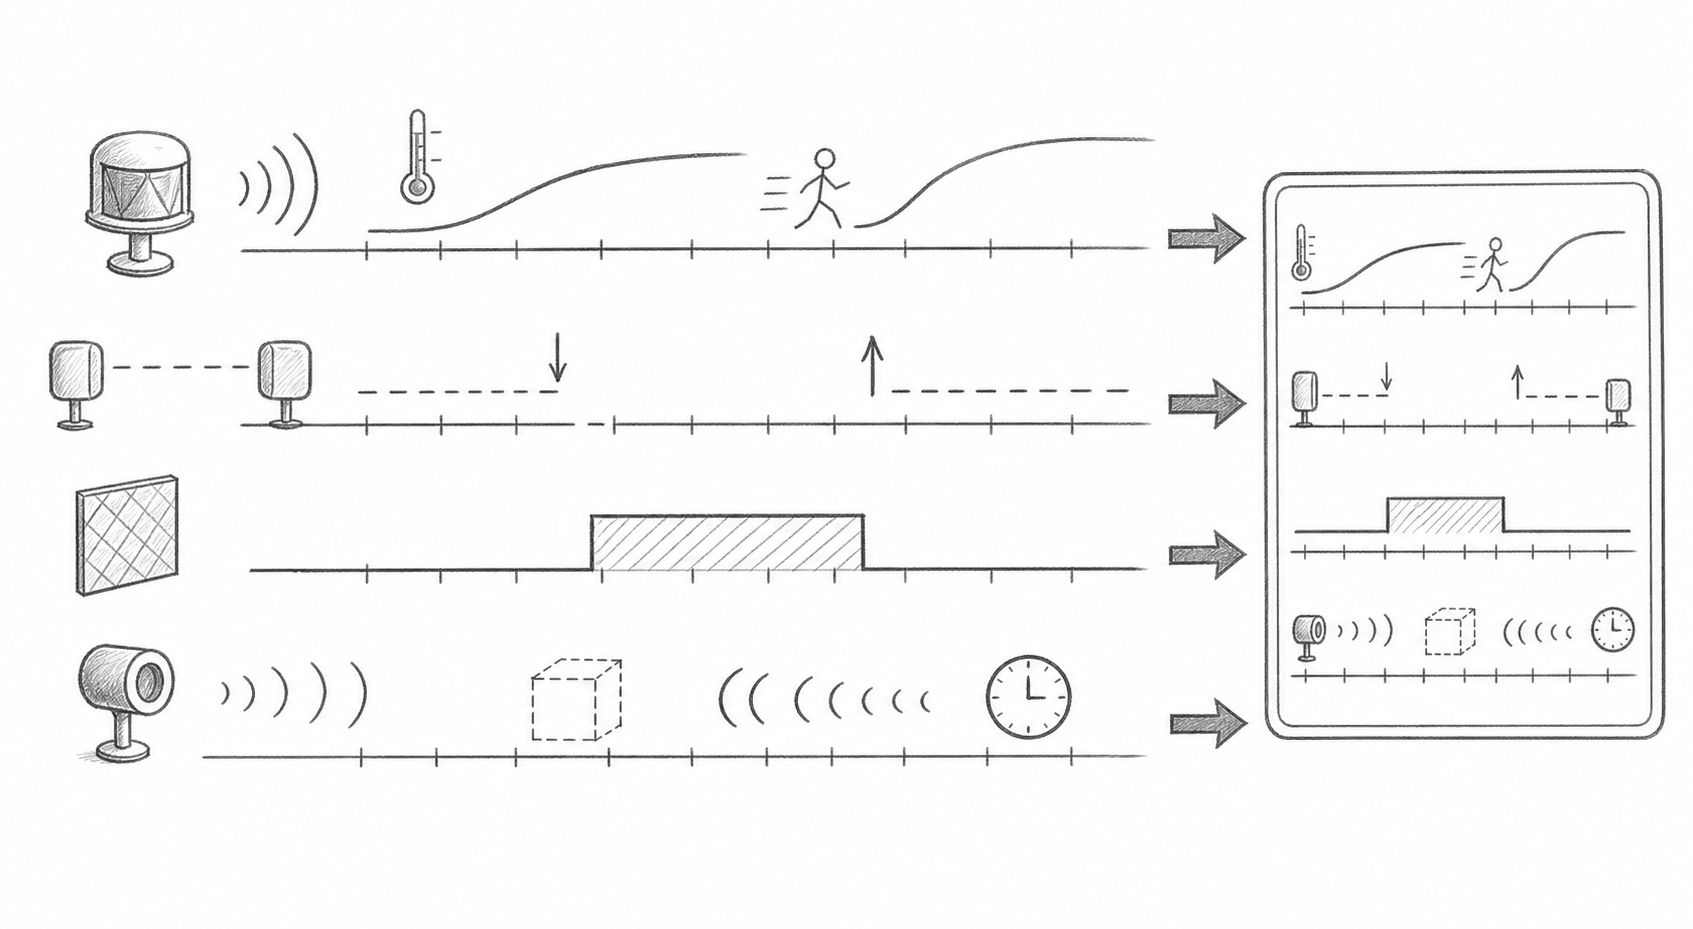
\includegraphics[width=0.98\linewidth]{041-evidence-lanes-pencil.png}

\small\textit{Alternative text: four hand-drawn timelines retain separate PIR,
beam, reflective-marker, and ultrasonic histories before entering one copied
evidence frame. Their different event epochs show that the values are not
assumed simultaneous.}
\end{center}

\texttt{PirObservationPolicy} qualifies copied digital samples. Warm-up must
finish before motion becomes eligible. Continuous qualified motion can become
\texttt{StuckMotion}; that is retained evidence, not proof that a person is
present. Clear and recovery use independent dwell intervals.

\texttt{PresenceModel} accepts already-qualified PIR and optical values plus a
copied \texttt{TimedRangeEvidence}. It does not resample, requalify, vote, or
replace a source. The E0 policies own no endpoint, claim, bus, timer,
interrupt, emitter, heap, callback, or hidden clock.

\begin{tabularx}{\linewidth}{@{}l X@{}}
\toprule
Retained evidence & Meaning\\
\midrule
PIR phase, epoch, age & warm-up, clear, motion, stuck motion, or source fault\\
beam provenance and edges & qualified interruption and restoration evidence\\
finish-guard provenance & calibration-bound reflective evidence from Lesson 040\\
range acquisition and copy epochs & measurement interval remains distinct from course time\\
quality, status, and age & old evidence remains stale rather than becoming false\\
\bottomrule
\end{tabularx}

\section{Age is part of the value}
Every present source epoch must be at or before the supplied frame time under
unsigned modular subtraction, and its age must stay below half-range. A future
epoch, exact half-range, or larger apparent age is a timing fault before
ordinary mutation.

A required absent source yields \texttt{Unqualified} with an Ok status; absence
is not invented hardware failure. Present malformed evidence faults. Freshness
is evaluated per source, so one newer observation cannot refresh an older one.

Range evidence deliberately names two domains. The microsecond acquisition
interval is the pair
\begin{center}
\texttt{measurementStartedAt} and \texttt{measurementLatency}.
\end{center}
The course-clock fields \texttt{startedAt} and \texttt{completedAt} identify
when acquisition began and when the terminal outcome was copied. A completion
stamp does not move the measurement epoch or pretend it was simultaneous with
newer optical evidence.

\section{Agreement is not a vote}
Each configured agreement source contributes one boolean claim only after it
is present, fresh, and valid. If the selected claims differ continuously
through \texttt{agreementWindow}, the snapshot becomes
\texttt{Disagreement}. Matching evidence clears that candidate. Missing,
stale, or faulted required evidence keeps its own higher-priority
classification instead of being mislabeled disagreement.

\begin{center}
% ADK visual: pencil
\begin{overpic}[width=0.78\linewidth]{041-passage-experiment-pencil.png}
 \put(2,44){\small hand-moved card}
 \put(2,33){\small warm-up then eligible}
 \put(2,23){\small interruption / restoration}
 \put(2,13){\small source-age comparison}
 \put(2,3){\small agreement / disagreement}
\end{overpic}

\small\textit{Alternative text: a hand moves an inert card between conceptual
gate posts while separate motion, beam, age, and agreement timelines remain
visible below. The drawing is orientation evidence, not wiring guidance.}
\end{center}

\section{One bounded passage event}
A passage candidate begins only on a valid beam interruption. A valid
restoration emits one \texttt{passageEvent} when it closes that candidate
after positive time no greater than \texttt{beamPassageWindow}, while the
complete required frame is fresh, valid, and not disagreeing. A long, stale,
faulted, or disagreeing frame clears the candidate without emitting.

The beam owns the transition. PIR, finish-guard, and range values remain
explicit context rather than a hidden majority vote. A repeated identical
source event is deduplicated by its typed identity, provenance, event kind,
and timestamp.

\section{Four-frame predict, observe, interpret}
\begin{enumerate}
 \item Keep the canonical sketch in replay mode. Predict two clear frames, one
       active frame, then one restoration frame. The sketch supplies
       already-qualified \texttt{ReadyClear}, \texttt{Motion}, and
       \texttt{ReadyClear} PIR observations; it does not run PIR warm-up.
 \item Observe D30 turn on only after both LED resources and the policy
       initialize. This is the acquisition signal. Observe D31
       (\texttt{TP-PRESENCE}) remain off for the first two clear frames, turn
       on for the active frame, and remain on for the restoration frame's
       passage event.
 \item In the active frame, predict PIR eligibility, beam interruption,
       finish-guard activation, and a 250 mm valid approach. D31 presents their
       combined state; it does not identify which source is active.
 \item In the restoration frame, predict clear PIR, restored beam, inactive
       guard, and 800 mm range, plus exactly one \texttt{passageEvent}. D31
       remains on as passage evidence.
\end{enumerate}

D30 and D31 each drive one LED through 1 k\(\Omega\) to ground in the
documented E1 presentation. D31 is selected off before policy initialization
and shuts down to high impedance on the fault path. Resource acquisition and
electrical safe state remain separate observations. The volatile
\texttt{evidenceCell}, \texttt{qualityCell}, and \texttt{rangeCell} are
debugger-readable supporting detail, not additional non-Serial indicators.

\section{Troubleshooting tree}
\begin{enumerate}
 \item \textbf{Unqualified:} identify the required absent source. Do not call
       absence a hardware fault.
 \item \textbf{Stale:} compare each source epoch with the frame epoch. Do not
       refresh old evidence by copying it again.
 \item \textbf{Disagreement:} inspect all selected claims and their ages. Do
       not choose a winner.
 \item \textbf{Source fault:} preserve the original status and source identity.
 \item \textbf{Timing fault:} check future, half-range, backward, and changed
       same-time evidence before interpreting physical meaning.
 \item \textbf{No passage event:} check interruption history, positive
       duration, passage window, freshness, and disagreement in that order.
\end{enumerate}

\section{Open powered and acceptance record}
\begin{tabularx}{\linewidth}{@{}p{0.48\linewidth}p{0.48\linewidth}@{}}
\toprule
Required evidence & Record\\
\midrule
Exact markings, revision, and authoritative source for each specimen & \rule{0.42\linewidth}{0.4pt}\\
Pin order, supply, rails, polarity, pull-ups, emitter, and current & \rule{0.42\linewidth}{0.4pt}\\
Aggregate pin, current, cadence, SRAM, flash, and stack result & \rule{0.42\linewidth}{0.4pt}\\
Resource acquisition prediction / observation / interpretation & \rule{0.42\linewidth}{0.4pt}\\
Named test-point safe state after shutdown & \rule{0.42\linewidth}{0.4pt}\\
Board revision, instruments, tool version, date, and commit & \rule{0.42\linewidth}{0.4pt}\\
\bottomrule
\end{tabularx}

\lessonbox{\textbf{Leave every row blank until measured.} Compilation,
synthetic replay, a pencil drawing, and this document do not establish
specimen conformance, electrical safety, powered behavior, or bench
acceptance. Resource acquisition and safe electrical state require separate
observations.}

\section{Software evidence and next use}
Host tests exercise PIR warm-up, retrigger, stuck-motion recovery, every
freshness boundary, disagreement, passage, completed-range tuple validation,
same-time identity, rollover, half-range rejection, reset, and field-stable
replay. Those are host-test exercises, not behavior demonstrated by the
four-frame sketch. The E0 object gate measures \texttt{PresenceModel} at
exactly 128 AVR bytes. The canonical Mega replay measures 8,818 bytes flash and
226 bytes static SRAM with the pinned AVR toolchain. Powered aggregate SRAM,
stack, pin, current, and cadence evidence remains open.

Lesson 042 may consume the snapshot as course evidence. Its explicit debounced
button press remains the sole start authorization; PIR motion can establish
eligibility but can never start a run.

This untagged print edition has a searchable HTML alternative.
It makes no PDF/UA or physical accessibility claim.
\end{document}
